\subsubsection{Begreper}
Positivt/negativt maksimum: Høyeste verdi i hver retning. \\
Periode: Tid fra starten av en bølge til starten av neste. \\
Peak voltage $V_P$: Den største spenningen målt fra null. \\
Peak to peak voltage $V_{PP}$: Spenningen mellom topp og bunn. \\
\\
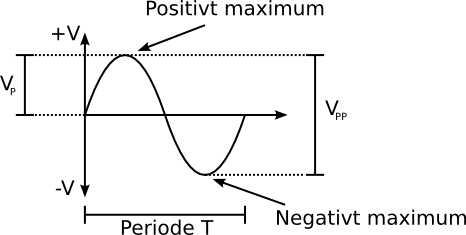
\includegraphics[width=\textwidth]{./img/veksel}

\subsubsection{Root mean square}
RMS brukes for å beregne gjennomsnitt til en AC-krets,
eller hva den samme spenningen ville tilsvare i en DC-krets.
\\\\
For eksempel har vi i norske stikkontakter vekselstrøm på 240 volt rms,
med peak voltage på 339 volt.
Det vil si at for å få samme effekt med DC må vi ha 240 volt.
\\\\
Effektverdi, rms, er gitt ved
$$V_{RMS} = \frac{V_P}{\sqrt{2}}$$
Der $V_P$ er peak verdien i AC-kretsen.
